\documentclass[12 pt, oneside]{article}
\textheight 9 in
\textwidth 6.5 in
\topmargin 0 in
\oddsidemargin .3 in
\evensidemargin .3 in
\usepackage{amssymb}
\usepackage{amsmath,amsthm}
\usepackage{amsbsy,paralist}
\usepackage{appendix}
\usepackage{natbib}
\usepackage{amsfonts}
\usepackage{graphicx}
\usepackage{epsfig}
\usepackage{color}
\usepackage{mathrsfs}
\usepackage{fancyhdr}
\usepackage{setspace}
%\usepackage[nodisplayskipstretch]{setspace}
\usepackage{fullpage}
\usepackage{cancel}
\usepackage{lipsum}
\usepackage{subfig}
\let\oldemptyset\emptyset
\let\emptyset\varnothing
\setlength{\parindent}{1cm}
\newtheorem*{thm}{Theorem}
\newtheorem*{lem}{Lemma}
\newtheorem{lemma}{Lemma}[section]
\newtheorem{lemfull}{Lemma}[section]
\newtheorem*{cor}{Corollary}
\newtheorem{corollary}{Corollary}[section]
\newtheorem{theorem}{Theorem}[section]
\newtheorem{thmfull}{Theorem}[section]
\newtheorem*{prop}{Proposition}
\newtheorem{proposition}{Proposition}[section]
\newtheorem{propfull}{Proposition}[section]
\theoremstyle{definition}
\newtheorem*{remark}{Remarks}
\theoremstyle{definition}
\newtheorem*{eg}{Example}
\theoremstyle{definition}
\newtheorem*{defn}{Definition}
\newtheorem{definition}{Definition}[section]
\newcommand{\bigsum}[2]{\sum\limits_{#1}^{#2}}
\newcommand{\bigprod}[2]{\prod\limits_{#1}^{#2}}
\newcommand{\nlim}{\lim_{n\ra\infty}}
\newcommand{\vecx}{\vec{x}}
\newcommand{\vecy}{\vec{y}}
\DeclareMathOperator{\Char}{Char}
\DeclareMathOperator{\orb}{orb}
\DeclareMathOperator{\stab}{stab}
\DeclareMathOperator{\Aut}{Aut}
\DeclareMathOperator{\Inn}{Inn}
\DeclareMathOperator{\lcm}{lcm}
\DeclareMathOperator{\card}{card}
\DeclareMathOperator{\Cl}{Cl}
\DeclareMathOperator{\Int}{Int}
\DeclareMathOperator{\var}{Var}
\DeclareMathOperator{\io}{i.o.}
\DeclareMathOperator{\sgn}{sgn}
\DeclareMathOperator{\tr}{trace}
\newcommand{\bfc}{\mathbf{c}}
\newcommand{\bfb}{\mathbf{b}}
\newcommand{\bfa}{\mathbf{a}}
\newcommand{\bfd}{\mathbf{d}}
\newcommand{\bff}{\mathbf{f}}
\newcommand{\bfh}{\mathbf{h}}
\newcommand{\bfg}{\mathbf{g}}
\newcommand{\bfi}{\mathbf{i}}
\newcommand{\bfj}{\mathbf{j}}
\newcommand{\bfk}{\mathbf{k}}
\newcommand{\bfl}{\mathbf{l}}
\newcommand{\bfm}{\mathbf{m}}
\newcommand{\bfn}{\mathbf{n}}
\newcommand{\bfo}{\mathbf{o}}
\newcommand{\bfp}{\mathbf{p}}
\newcommand{\bfq}{\mathbf{q}}
\newcommand{\bfr}{\mathbf{r}}
\newcommand{\bfs}{\mathbf{s}}
\newcommand{\bft}{\mathbf{t}}
\newcommand{\bfx}{\mathbf{x}}
\newcommand{\bfy}{\mathbf{y}}
\newcommand{\bfz}{\mathbf{z}}
\newcommand{\bfu}{\mathbf{u}}
\newcommand{\bfv}{\mathbf{v}}
\newcommand{\bfw}{\mathbf{w}}
\newcommand{\bfX}{\mathbf{X}}
\newcommand{\bfY}{\mathbf{Y}}
\newcommand{\bfA}{\mathbf{A}}
\newcommand{\bfB}{\mathbf{B}}
\newcommand{\bfC}{\mathbf{C}}
\newcommand{\bfD}{\mathbf{D}}
\newcommand{\bfE}{\mathbf{E}}
\newcommand{\bfF}{\mathbf{F}}
\newcommand{\bfG}{\mathbf{G}}
\newcommand{\bfH}{\mathbf{H}}
\newcommand{\bfI}{\mathbf{I}}
\newcommand{\bfJ}{\mathbf{J}}
\newcommand{\bfK}{\mathbf{K}}
\newcommand{\bfL}{\mathbf{L}}
\newcommand{\bfU}{\mathbf{U}}
\newcommand{\bfV}{\mathbf{V}}
\newcommand{\bfW}{\mathbf{W}}
\newcommand{\bfZ}{\mathbf{Z}}
\newcommand{\bfM}{\mathbf{M}}
\newcommand{\bfN}{\mathbf{N}}
\newcommand{\bfQ}{\mathbf{Q}}
\newcommand{\bfO}{\mathbf{O}}
\newcommand{\bfR}{\mathbf{R}}
\newcommand{\bfS}{\mathbf{S}}
\newcommand{\bfT}{\mathbf{T}}
\newcommand{\bfP}{\mathbf{P}}
\newcommand{\bfzero}{\mathbf{0}}
\newcommand{\R}{\mathbb{R}}
\newcommand{\E}{\mathbb{E}}
\newcommand{\N}{\mathbb{N}}
\newcommand{\Q}{\mathbb{Q}}
\newcommand{\Z}{\mathbb{Z}}
\newcommand{\curA}{\mathscr{A}}
\newcommand{\curC}{\mathscr{C}}
\newcommand{\curD}{\mathscr{D}}
\newcommand{\curE}{\mathscr{E}}
\newcommand{\curH}{\mathscr{H}}
\newcommand{\curI}{\mathscr{I}}
\newcommand{\curJ}{\mathscr{J}}
\newcommand{\curK}{\mathscr{K}}
\newcommand{\curN}{\mathscr{N}}
\newcommand{\curO}{\mathscr{O}}
\newcommand{\curQ}{\mathscr{Q}}
\newcommand{\curS}{\mathscr{S}}
\newcommand{\curT}{\mathscr{T}}
\newcommand{\curU}{\mathscr{U}}
\newcommand{\curV}{\mathscr{V}}
\newcommand{\curW}{\mathscr{W}}
\newcommand{\curZ}{\mathscr{Z}}
\newcommand{\curB}{\mathscr{B}}
\newcommand{\curF}{\mathscr{F}}
\newcommand{\curG}{\mathscr{G}}
\newcommand{\curM}{\mathscr{M}}
\newcommand{\curL}{\mathscr{L}}
\newcommand{\curP}{\mathscr{P}}
\newcommand{\curR}{\mathscr{R}}
\newcommand{\curX}{\mathscr{X}}
\newcommand{\curY}{\mathscr{Y}}
\newcommand{\calA}{\mathcal{A}}
\newcommand{\calD}{\mathcal{D}}
\newcommand{\calF}{\mathcal{F}}
\newcommand{\calK}{\mathcal{K}}
\newcommand{\calO}{\mathcal{O}}
\newcommand{\RA}{\Rightarrow}
\newcommand{\ra}{\rightarrow}
\newcommand{\fd}{\vspace{2.5mm}}
\newcommand{\as}{\vspace{1mm}}
\title{A Brief Introduction to HACT and HANK}
\author{William Chen and Emily Martell}
\date{August 6, 2018}

\begin{document}
\maketitle
\abstract{This paper explains, in moderate detail, the set up of HACT models (e.g. HANK). We cover the basic mathematics behind the steady state solution and the linear approximation methods used in Ahn et al. (2017), assuming only preliminary knowledge of stochastic continuous-time methods. Next, we discuss methods of implementing an estimation with HANK models. We conclude with potential paths for future work, both of theoretical interest and of policy interest.}



\section{Steady State Theory}
Individual consumers face the problem
\begin{equation}
\rho v_t = \max_c u(c) + \dfrac{1}{dt}\E[dv_t]
\label{hjb}
\end{equation}
subject to the dynamic budget constraint
\begin{equation}
\label{wealth law of motion}
da_t = \left(w_tz_t + ra_t - c_t\right)\,dt.
\end{equation}
Generically, $z_t$ is agents' idiosyncratic labor productivity and follows some stochastic process (in Krusell Smith, we have a continuous-time Markov chain). The first equation is just the Hamilton-Jacobi-Bellman equation, which is the continuous-time equivalent of the Bellman equation for discrete-time dynamic programming. In equilibrium, $v_t$ will depend on a variety of state variables depending on the modeled heterogeneity and aggregate shocks.

We can partition the state variables into two categories: idiosyncratic and aggregate. Using this distinction, for standard stochastic processes, we can simplify \eqref{hjb} to
\begin{equation}\label{hjb simplified}
\rho v_t = \max_c u(c) + \calA v_t + \dfrac{1}{dt}\E_t[dv_t],
\end{equation}
where $\calA$ is the generator\footnote{Technically, it is just known as the transition matrix, but to simplify the number of terms, we make the slight abuse of terminology and still say generator.} of the stochastic process describing the evolution of idiosyncratic states. For example, if the idiosyncratic states follow a Brownian motion, then the generator $\calA$ is the Laplacian. Observe that the expectation operator becomes $\E_t$ to reflect that the expectation only applies now to aggregate states, i.e. it is a conditional expectation w.r.t. aggregate states.

Under certain conditions, there exists a potentially time-varying probability distribution over \textit{idiosyncratic} states that solves the Kolmogorov Forward/Fokker-Planck equation
\begin{equation}  \label{kfe}
\dfrac{dg_t}{dt} = \calA^*g_t,
\end{equation}
where $\calA^*$ is the adjoint of the generator $\calA$\footnote{For details, consult a functional analysis textbook/lecture notes on unbounded linear operators and their adjoints.}. The steady-state in our model is defined to be when the distribution $g_t$ no longer varies, i.e. the LHS of \eqref{kfe} equals zero.

The particular markets involved vary depending on the HACT model, but generically, we can summarize market-clearing conditions by the functional
\begin{equation}\label{market clearing}
\bfp_t = \calF(g_t),
\end{equation}
where $\bfp_t$ is a vector of prices.

To solve for the steady state, we need to approximate these functions on a discrete grid. In the steady state, $\E_t[dv_t] = 0$, so we may neglect this term. Letting boldface variables denote the discretized representation of functions, we have
\begin{align*}
\rho \bfv & = \bfu(\bfv) + \bfA(\bfv;\bfp)\bfv\\
\bfzero & = \bfA(\bfv;\bfp)^T\bfg\\
\bfp & = \bfF(\bfg),
\end{align*}
where we ignore time subscripts since this is a steady state. Here, $\bfA$ is the matrix approximation of the generator $\calA$, and the adjoint of $\calA$ becomes just the transpose in the matrix representation\footnote{It can be shown that the adjoint of a generator is similar to the transpose of the generator, and in the finite-dimensional case, this property reduces to the adjoint of a generator being its transpose. See wikipedia's article on unbounded linear operators.}. Solving for the steady-state can be accomplished with a variety of schemes, but the most common one is finite differences since this matrix representation is essentially a PDE system.

Having solved for the steady state, we can now consider the approximated aggregate system:
\begin{align*}
\rho \bfv_t & = \bfu(\bfv_t) + \bfA(\bfv_t;\bfp_t)\bfv_t + \dfrac{1}{dt}\E_t[d\bfv_t]\\
\dfrac{d\bfg_t}{dt} & = \bfA(\bfv_t;\bfp_t)^T\bfg_t\\
\bfp_t & = \bfF(\bfg_t),\\
dZ_t & = \eta Z_t\,dt + \sigma\, dW_t,
\end{align*}
where $Z_t$ is a vector of aggregate state variables, assumed to follow a linear Ito diffusion (although this need not be the case). In this case, the cross-sectional distribution $g_t$ varies with the aggregate shocks, as do all the other variables, hence the return of the time subscripts. Solving this PDE system would be prohibitively difficult because we would need to solve for the behavior of $g_t$ as a function of aggregate variables.

Instead, we linearize this system around the steady state. Prior to linearization, we re-write the aggregate system in the form
\begin{align*}
\E[d\bfv_t] & = \left[\rho \bfv_t -\bfu(\bfv_t)- \bfA(\bfv_t;\bfp_t)\bfv_t\right]\, dt\\
d\bfg_t & = \bfA(\bfv_t;\bfp_t)^T\bfg_t\, dt\\
dZ_t & = \eta Z_t\,dt + \sigma\, dW_t,
\end{align*}
where we remove the market-clearing equations since these are statically solved and can be directly substituted into the other equations. On the LHS, we only have differentials, and on the RHS, all the variables depend on the levels of $\bfv_t, \bfg_t, \bfp_t$, and $Z_t$. We can therefore represent the LHS as
\begin{equation}
  \begin{bmatrix}
    \E[d\bfv_t]\\d\bfg_t\\dZ_t
  \end{bmatrix} = \bff(\bfv_t;\bfg_t;\bfp_t;Z_t),
\end{equation}
where $\bff(\cdot) = \bfzero$ in the steady state. Our linearization approximates this nonlinear function $\bff$ by taking first-order derivatives w.r.t. $\bfv_t, \bfg_t, \bfp_t$, and $Z_t$ evaluated at the steady state. After linearization and placed in gensys canonical form, we have the linear system
\begin{equation}\label{linearized system}
  \begin{bmatrix}
    \E[d\hat{\bfv}_t]\\d\hat{\bfg}_t\\dZ_t
  \end{bmatrix} = \Gamma_1
  \begin{bmatrix}
    \hat{\bfv}_t\\\hat{\bfg}_t\\ Z_t
  \end{bmatrix} + \Psi\, dW_t + \Pi\, \eta_t + C
\end{equation}
where the hats denote the fact that these variables are expressed as steady-state deviations due to linearization. Generally, as can be seen from the system before linearization, we will have $C = 0$. Moreover, in our model the expectational errors only arise from expectations of the value function, so it will be the case that $\eta_t$ will capture expectational errors of the value function rather than any of the other variables. In particular, in this model, $\hat{\bfg}_t$ is assumed to be observed perfectly as an aggregate state variable.

\section{Finite Difference Methods}
We only give a brief description here of the finite difference methods used to solve the value function PDE. A more detailed description is given in Achdou et al. (2017). Basically, suppose we have some differentiable function $f:\R\ra\R$ and a grid of points $x_0,\dots, x_n$. We can approximate a first-order derivative as
\begin{equation}
\label{eq:ex first order finite difference}
  \dfrac{d f(x_i)}{d x} \approx \dfrac{f(x_{i+1}) - f(x_i)}{(x_{i+1} - x_i)}.
\end{equation}
This is called a forward difference because we are approximating the derivative of $f$ evaluated at $x_i$ by using the value of $f$ one ``step'' ahead, i.e. $f(x_{i+1})$. A backward difference can similarly be defined by using $f(x_i) - f(x_{i-1})$ for the numerator. This same method can be used to approximate partial derivatives since we're basically using the limit definition of derivatives.

We can similarly approximate higher order derivatives, and there are certain recommended formuals for these approximations. For example, a second-order forward difference is recommended to be computed as
\begin{equation}
\label{eq:ex second order finite difference}
  \dfrac{d f(x_i)}{d x} \approx \dfrac{f(x_{i+2}) - 2f(x_{i+1}) + f(x_i)}{(x_{i+2} - x_{i+1})(x_{i+1} - x_i)}.
\end{equation}
This recommendation is related to minimizing the order of the error introduced because we are not taking the limit to zero.

An upwind scheme for finite differences is supposed to guarantee that certain conditions, which theoretically imply convergence of a finite difference scheme toward the solution of a PDE, are satisfied. The basic idea is that if the drift in the state variable is possible, use a forward difference, and if it is negative, then use a backward difference. For example, consider wealth. The drift of wealth is positive when savings is positive since positive savings imply wealth accumulation. When an agent is dissaving, the drift of wealth is negative, implying wealth deccumulation. Thus, the upwind scheme uses a forward difference to the value function whenever an agent is predicted to be net saving at a given point and a backward difference when the agent is net dissaving.

\section{Krylov Subspace Methods and Reduction of State Variables}
Here, we describe only the basis reduction with exogenous decision rules. We have yet to implement the internal consistency check that allows for endogenous decision rules. In addition, we only explain here briefly how Krylov reduction works. See Ahn et al. (2017) for a detailed explanation of why we use Krylov reduction to choose a basis to span the subspace generated by the observability matrix associated with our linearized system. Basically, given our distribution vector $\hat{\bfg}_t$ and any additional state variables $Z_t$, we want to find a basis for a lower dimensional subspace $S$ such that
\[
\begin{bmatrix}
  \hat{\bfg}_t\\Z_t
\end{bmatrix} \approx \bfX_\gamma \gamma_t,
\]
where $\gamma_t\in S$. To achieve a good approximation, we use subspace spanned by the order-$k$ observability matrix associated with our linearized system and attempt to project onto that subspace. In particular, we may represent our expected linearized system \eqref{linearized system} as
\[ \E \begin{bmatrix}
    \E[d\hat{\bfv}_t]\\d\hat{\bfg}_t
  \end{bmatrix} =
  \begin{bmatrix}
    \bfB_{vv} & \bfB_{vp} \bfB_{pg} & \bfB_{vp}\bfB_{pz}\\
    \bfB_{gb} & \bfB_{gg} + \bfB_{gp}\bfB_{pg} & \bfB_{gp} \bfB_{pZ}
  \end{bmatrix}
  \begin{bmatrix}
    \hat{\bfv}_t\\\hat{\bfg}_t\\ Z_t
  \end{bmatrix}.
\]
It can be shown that our desired observability matrix is $\calO(\bfB_{pg}, \bfB_{gg} + \bfB_{gp}\bfB_{pg})^T$, and it turns out that the observability matrix is precisely an order-$k$ Krylov subspace, which is defined as
\[ \calK_k(\bfA,\bfb) = \text{span}(\{\bfb, \bfA\bfb, \bfA^2\bfb,\dots, \bfA^{k-1}\bfb\}), \]
for some $N\times N$ matrix $\bfA$ and $N\times 1$ vector $\bfb$. In particular, we want to project onto the Krylov subspace
\[\calK_k(\bfB_{gg}^T + \bfB_{gp}^T\bfB_{pg}^T, \bfB_{pg}^T).  \]
Direct regression onto this subspace is not numerically stable to multiple collinearity, as the basis which defines a Krylov subspace is a polynomial. Instead, there exist many other methods for projecting onto this space.

We now summarize the Krylov reduction step in our framework in two primary steps. First, we take our linearized system \eqref{linearized system} and partition our $\Gamma_1$ matrix into particular blocks (see the paper for the exact partition). Using those blocks, it can be shown that the desired observability matrix can be represented as an order-$k$ Krylov subspace based off those block matrices. Second, to find the basis projection into this Krylov subspace, we may use deflated block Arnoldi iteration, which has two advantages. One, it is a stable way to orthogonalize the basis. Two, it handles multicollinearity well by using deflation.


\section{Spline Basis Projection and Reduction of the Value Function}
Assuming the $\hat{\bfv}_t$ is approximately smooth\footnote{Observe we are talking about the deviations from the steady state; we do not need the actual steady state value function to be everywhere differentiable, allowing us to capture non-convexities. We just need that the deviations from the steady state are non-smooth at a finite number of points, and then splines should be fine.}, we can use splines as an approximation. In particular, we may write any spline approximation as the projection
\begin{equation}
  \label{spline projection}
\hat{\bfv}_t \approx \bfX_\nu \nu_t,
\end{equation}
where $\bfX_\nu$ is a matrix performing a change of basis from the original state space grid describing the heterogeneity of agents into a spline basis, where $\bfX_\nu$ defines a linear combination of spline knot points and $\nu_t$ are the coefficients at those knot points. Quadratic splines are chosen to maintain monotonicity and concavity between knot points. For more details why we choose splines, see Ahn et al. (2017). To construct this basis, we a priori choose a number of knot points in the state space, and it is advised that these knot points be non-uniform. We then use the actual state space grid and these knot points as the coordinates the change of basis should map to and from, i.e. if $\bfx$ are the actual state space grid points and $\bfk_t$ are the knot points, then $\bfx = \bfX_\nu \bfk_t$. For more details about how to implement the spline projection, see the Julia code.

To get some intuition for why this is the way we construct $\bfX_\nu$, think of $\bfx$ as representing particular standard basis vectors in $\R^n$ space, where $n$ is the dimension of $\bfv_t$. The actual function $v_t$ lives in a function space, but we approximate in a finite-dimensional Euclidean subspace at particular ``dimensions'' in the infinite-dimensional representation of $v_t$. For example, the wealth grid point corresponding to $a = 0$ can be thought of as the ``first'' dimension in $\R^n$ space and is therefore just the $e_1$ standard basis vector. The value of $\bfv_t$ at $a = 0$ can be interpreted as a scalar multiple of $e_1$. Similarly, when we approximate $\hat{\bfv}_t$ with splines, we are trying to represent an infinite-dimensional object in a finite vector space. In this spline vector space, the basis vectors are the knot points of the splines, so the basis transformation matrix $\bfX_\nu$ must map the coordinates of the wealth grid to the knot points because $\bfX_\nu$ takes basis vectors to basis vectors.

\section{Description of KrusellSmith and OneAssetHANK}
\subsection{KrusellSmith}
KrusellSmith is essentially a basic RBC model with a Bewley-Aiyagari structure for the consumption-saving problem, perfectly inelastic labor supply, and aggregate productivity shocks. This subsection first describes the consumption-savings problem faced by heterogeneous households and then the production side.

Preferences for agent $j$ are given by standard CRRA utility:
\[\E_0\left[\int_0^\infty e^{-\rho t}\dfrac{c_{jt}^{1-\gamma}}{1-\gamma}\,dt \right], \]
where $\rho$ is the rate of time preference and $\gamma$ the coefficient of relative risk aversion. In the steady-state, agent $j$'s wealth follows
\[\dot{a}_t =  w_t z_{jt} + r_ta_t -c_t \]
where $z_{jt}\in \{z_L, z_H\}$, with $z_L< z_H$, moves according to a Poisson process with arrival rates $\lambda_L$ and $\lambda_H$. All agents are assumed to supply a single unit of labor, hence the perfect inelasticity of labor supply. Agents also face the borrowing constraint $a_{jt}\geq 0$, and markets are incomplete because agents may only trade their wealth $a_{jt}$, cannot insure away idiosyncratic shocks, and cannot write Arrow securities on aggregate states. Finally, capital is the only source of wealth, so for each unit of wealth, agents can supply a unit of capital and earn the rental rate $r_t$.

A representative firm aggregates the supply of labor and capital/wealth via the Cobb-Douglas function
\[ Y_t = e^{Z_t}K_t^\alpha N_t^{1-\alpha}, \]
where $Z_t$ is the logarithm of aggregate productivity, $K_t$ is aggregate capital, and $N_t$ is aggregate labor. $Z_t$ is assumed to follow a mean-reverting Ornstein-Uhlenbeck process, which creates stationarity. See Ahn et al. (2017) for the full set of equilibrium conditions.

To summarize, due to idiosyncratic labor income shocks, borrowing constraints, and incomplete markets, households are heterogeneous in their income and wealth, so aggregate quantities and prices depend on the cross-sectional distribution of households in their income and wealth levels. The model has no money nor nominal rigidities, so it is a real-business cycle model with a perfectly competitive production sector.



\subsection{OneAssetHANK}
For the full description, go to the top level directory of EHANK and see /matlab/phact/examples/one\_assset\_HANK/docs/one\_asset\_hank\_no\_capital.pdf. Here, we go into even less detail. This model is effectively a New-Keyensian model with income and wealth heterogeneity, a central bank, and fiscal policy. Preferences are the standard CRRA utility over consumption with separable labor disutility:
\[\E_0\left[ \int_0^\infty e^{-\rho t}\left(\dfrac{c_t^{1-\gamma}}{1-\gamma} - \phi_0\dfrac{l_t^{1+1/\phi_1}}{1+1/\phi_1}\right)\,dt \right]. \]
Income again evolves according to a Poisson process like in KrusellSmith, and households are taxed on their labor earnings, earn a lump-sum transfer from the government, and earn profits from firms proportional to income (since households are assumed to own firms). The model only has a single asset, which are government bonds, and all wealth is held in government bonds\footnote{In the two-asset HANK model, agents can hold illiquid assets, which are interpreted as equity shares in firms, so profits are distributed only to holders of illiquid asset.}. Individual agents face the borrowing constraint $a_{jt}\geq \underline{a}$.

Production has a final good CES aggregator and a monopolistically competitive intermediate goods sector. Nominal rigidities are generated by Rotemberg pricing (quadratic adjustment costs to price-resetting), making space for monetary policy, which is assumed to follow a Taylor Rule with moentary policy shocks (the only source of aggregate shocks in this model):
\[i_t = \overline{r}_t + \phi_\pi\pi_t + \phi_y(y - \overline{y}) + \varepsilon_{MP,t},  \]
where the monetary policy shock evolves according to a mean-reverting Ornstein-Uhlenbeck
\[d\varepsilon_t = -\theta_{MP}\varepsilon_t\,dt + \sigma_t\cdot dW_t.  \]
The government's income is given by taxes raised and interest on government bonds outstanding. The government's expenditures are on spending $G_t$, transfers $T_t$, and changes in bonds outstanding $\dot{B}_t^g$.

\subsection{Timing Results}
KrusellSmith
  \begin{center}
    \begin{tabular}{|c|c|c|}
      \hline
      Code Section & Julia & Matlab\\
      \hline
      All, Do Checks & 239 ms & 234 ms\\
      All, No Checks & 249 ms & ---\\
      steadystate! & 57.89 ms & 130 ms\\
      eqcond & 164.427 ms & 54.9 ms\\
      reduction & 11.43 ms & 33.525 ms\\
      gensys & 646$\mu$s & 9.09 ms\\
      gensys! & 5.53 ms & ---\\
      \hline
    \end{tabular}
    \begin{itemize}
    \item Do Checks: ensure mandatory settings defined, $\Gamma_0$ is identity, so not checking should be faster, right?
    \item eqcond is slower for some reason. Automatic differentiation was tested to be faster earlier though, right?
    \item gensys is faster when I don't use in-place Schur factorization. Ideas?
    \end{itemize}
  \end{center}

OneAssetHANK
  \begin{center}
    \begin{tabular}{|c|c|c|}
      \hline
      Code Section & Julia & Matlab\\
      \hline
      All, Do Checks & 1.097 s & 791.2 ms\\
      All, No Checks & 1.101 s & ---\\
      steadystate! & 547.767 ms & 537.8 ms\\
      eqcond & 414.913  ms & 240.07 ms\\
      reduction & 130.938 ms & 55.002 ms\\
      gensys & 2.503 ms & 11.852 ms\\
      gensys! & 2.606 ms & ---\\
      \hline
    \end{tabular}
\begin{itemize}
\item eqcond is substantially slower again
\item Reduction here is substantially slower, too
\item gensys! is still slower...
\end{itemize}
  \end{center}


\section{Estimation}
\subsection{Continuous-Time Kalman Filters}
In this section, we describe the two continuous-time Kalman filters we have implemented.

\subsubsection{Continuous-Time State with Discrete Observations}
This textbook\footnote{http://www.uta.edu/utari/acs/2015\%20robotics\%20SCUT/NEU\%20June\%20shorcourse\%20notes/Lewis-\%20Optimal\%20and\%20robust\%20estimation.pdf} in section 3.7 describes the scheme. Basically, our true transition and measurement equations are given by
\begin{align*}
  ds_t & = Ts_t\,dt + R\, dW_t\\
  y_\tau & = Zs_\tau + D + u_\tau,
\end{align*}
where $t\in [0,\infty)$ and $\tau \in \N$. In other words, our states occur in continuous time, but we only have discrete observables at some regular frequency described by $\tau$. To filter this, we take the expectation of the first equation to arrive at the deterministic ODE
\begin{align*}
  \dfrac{\E[ds_t]}{dt} & = Ts_t,
\end{align*}
which describes the expected change in $s_t$. Typically, the Kalman Filter is split into a prediction step and a update step. The first step does not depend on data and only on the transition equation. We replace the true transition equation with the deterministic ODE above, and we solve it as an initial value problem using some ODE integration routine like a Runge-Kutta method. The length of time used for integration will depend on the meaning of $\tau$. In our implementation, we assumed the length of time is just one, for one quarter.

The update step is the same as in the discrete time Kalman filter. This follows from the fact that with a Brownian motion as the source of variation in the state transition equation, we can treat the Brownian shock as if it occurs all at once in period $\tau$, and we can update as if we just had an instantaneous mean-zero normal shock.


\subsubsection{Simulated Subintervals with Discrete Observations}
This scheme uses the discrete-time Kalman filter but essentially expands the number of states we track. Let $\tau$ be the length of time in between discrete observations. Then we approximate the behavior of $s_t$ by subdividing the interval $[0,\tau]$ into subintervals and using an Euler-Maruyama scheme to guess how $s_t$ moves around. In particular, suppose we have $n$ subintervals. Then we say that
\[s_{t,i+1} = Ts_{t, i}\cdot\dfrac{\tau}{n} + R\epsilon_{t,i+1},\quad\text{for }i =0,1,2,\dots, n  \]
where $\epsilon_{t,i+1}\sim N(0, \frac{\tau}{n}I)$, $s_{t,0} = s_t$, and $s_{t,n} = s_{t+\tau}$. We then let our new ``state'' vector be
\[S_t =
\begin{bmatrix}
  s_{t,1}\\s_{t,2}\\.\\.\\.\\s_{t,n}
\end{bmatrix}
\]
and have the transformed state transition equation
\[S_{t+\tau} = TT\, S_t + RR\,\vec{\epsilon}_t, \]
where
\[TT =
\begin{bmatrix}
  0 & 0 & \cdots &  0 & (T+I)\\
0 & 0 & \cdots & 0 & (T+I)^2\\
\cdot & \cdot & \cdots & \cdot & \cdot\\
0 & 0 & \cdots & 0 & (T+I)^n
\end{bmatrix}
\]
and
\[RR =
\begin{bmatrix}
  R & 0 & 0 & \cdots & 0 & 0 \\
(T+I)R & R & 0 & \cdots & 0 & 0\\
(T+I)^2R & (T+I)R & R & \cdots & 0 & 0\\
\cdot & \cdot &  \cdot & \cdots & \cdot & \cdot\\
(T+I)^nR & (T+I)^{n-1}R & (T+I)^{n-2}R & \cdots & (T+I)R & R\\
\end{bmatrix}.
\]
To see how we construct these matrices, just note the recursive structure of our transition equation. Effectively, we are trying to filter for the path of $s_t$ while only having access to discrete observations.

Note that we must actually stack the entire state vector unless the user verifies that certain states are redundant. For example, suppose we wish to track flow output in KrusellSmith. Then the 404th row of the full $T+I$ matrix corresponds to the matrix multiplication that gives us the change. Generally, the entire row is nonzero

\subsection{Timing and Accuracy}
Here, we present some results on the timing and accuracy of these different methods. First, we describe the data-generation process. We use the model KrusellSmith to generate simulated data in the following manner.
\begin{enumerate}
\item Initialize $s_0 = \bfzero$, i.e. we start at the steady state.
\item Set $dt = 1/90$ for the Euler-Maruyama scheme so that 1 full period (a time step of 1) is a quarter, and each time step $dt$ is equivalent to a day.
\item To generate $N$ years of data, perform the following calculation $360\cdot N$ times:
\[s_{t+1} = (I + T\,dt)s_t + R \varepsilon_{t+1},  \]
where $T$ and $R$ are the transition matrices from the true state transition equation
\[ds_t = Ts_t\, dt + R\, dW_t,  \]
and $\varepsilon_{t+1}\sim N(0, dt * I)$, i.e. $\varepsilon_{t+1}$ is a mean-zero normal shock with variance $dt$, per shock.
\item Save the path of $s_t$, which generates $360\cdot N + 1$ data points.
\end{enumerate}
The following timing and accuracy results are performed by taking the entry in $s_t$ which corresponds to flow output, sampling from it every 90 days to create ``quarterly'' observations, and then applying the Kalman filter. The data itself is generated with $N = 50$ so that we obtain 50 years worth of data, which is roughly on the order we would imagine actual data to be. For KrusellSmith, our $Z$ matrix will be a $1\times 406$ matrix, and the 404th entry in $s_t$ tracks flow output. Therefore, our $Z$ matrix will be all zeros except for a one in the 404th location, so that $Zs_t$ returns the predicted flow output at each time when data is available (i.e. each quarter). We do not add any measurement noise. Heuristically, this exercise evaluates how well the Kalman filter can estimate the volatility of the true state transition process when it can only ``see'' the true state vector every 90th data point.

We report timing results first and then accuracy. The ODE integration method reports the type of integration scheme used, and the subintervals method type is reported as the number of simulated subintervals per quarter.
\begin{center}
  \begin{tabular}{|c|c|c|c|}
    \hline
    Method & Time (ms) & Allocations & Memory (MiB)\\
\hline
    ODE Integration - Euler & 418.813  & 440419 & 634.9 \\
    ODE Integration - Tsitouras 5/4 & 421.565 & 440019  & 634.89\\
    Subintervals - 2  & 50.181 & 15071 & 67.84 \\
    Subintervals - 3  & 126.252 & 15071 & 149.88\\
    Subintervals - 12 & 4601 & 16214 & 2300\\
\hline
  \end{tabular}
\end{center}
These results can be reproduced by using the julia file in the docs/kalman\_filter/timing folder of the EHANK repository.

The accuracy results are below. By mean absolute distance, we compute mean(max\_lik\_$\sigma$ - true\_$\sigma$), where max\_lik\_$\sigma$ is a vector holding the $\sigma$ predicted by MLE, and true\_$\sigma$ is the true parameter. The standard deviation of the error just takes std(max\_lik\_$\sigma$ - true\_$\sigma$), and the max absolute error is maximum(abs.(max\_lik\_$\sigma$ - true\_$\sigma$)).


\fd

Salient results: CT ODE integration method seems to be both (a) more accurate at inferring the true parameter on average and (b) greater precision (standard deviation of errors is smallest). We also get that the more subintervals which are included, the less accurate the simulated subintervals method is, although the precision does go up. This suggests to me that somewhere, something is getting coded incorrectly. My first guess for places to check are making sure the size of the fundamental shock and the time step dt are all correctly aligned. For example, the Brownian shock should have variance dt, not variance one, because of how Brownian motions are defined.


\begin{center}
\begin{tabular}{|c|c|c|c|}
\hline
Method &  Mean absolute distance & Std(error) & Max abs error\\
\hline
ODE Integration - Tsitouras 5/4 & .00122 & .0004855 & .00199\\
Subintervals - 2 &.00157 & .000438 & .00199\\
Subintervals - 3 & .00158 & .000436 & .00199\\
Subintervals - 12 & .00159 & .000423 & .00199\\
\hline
\end{tabular}
\end{center}


The grid of $\sigma$'s that we searched on was a uniform grid of 20 points from $\sigma = .005$ to $\sigma = .009$, and we manually inserted the truth of $\sigma = .007$. These results can be reproduced by using the files in docs/kalman\_filter called ct\_kalman\_filter.jl and sim\_kalman\_filter.jl in the EHANK repository.

Here are the histograms corresponding to the above results.
\begin{figure}[[h!]]
  \centering
  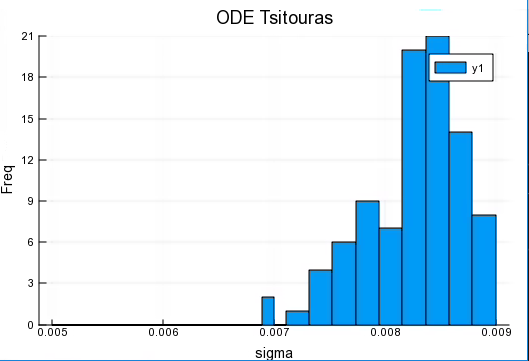
\includegraphics[width=.5\textwidth]{figures/ode_tsitouras_hist.PNG}
  \caption{ODE MLE Histogram}
\end{figure}
\begin{figure}[[h!]]
  \centering
  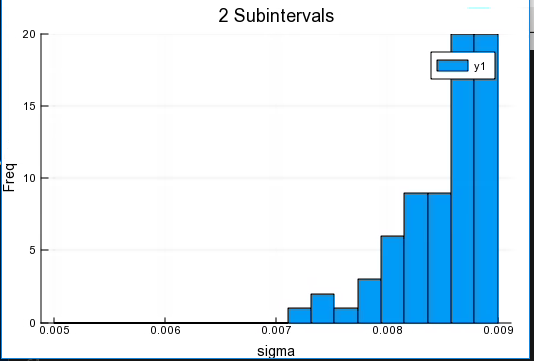
\includegraphics[width=.5\textwidth]{figures/2_subintervals_hist.PNG}
  \caption{2 Subintervals MLE Histogram}
\end{figure}
\begin{figure}[[h!]]
  \centering
  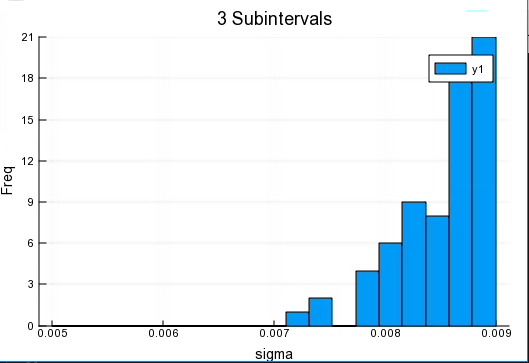
\includegraphics[width=.5\textwidth]{figures/3_subintervals_hist.PNG}
  \caption{3 Subintervals MLE Histogram}
\end{figure}
\begin{figure}[[h!]]
  \centering
  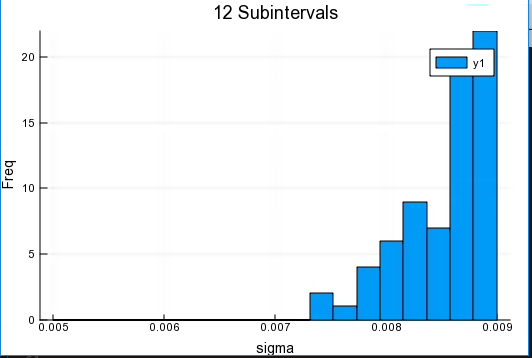
\includegraphics[width=.5\textwidth]{figures/12_subintervals_hist.PNG}
  \caption{12 Subintervals MLE Histogram}
\end{figure}




\subsection{Notes on Other Kalman Filters}
Here we briefly describe other Kalman filters we explored. In the estimate folder, we have two ``block'' Kalman filters. The BlockKalmanFilter type is an implementation of a block filter for large-scale DSGE models (read the paper referenced in the code description of this filter) and is intended to reduce the number of matrix multiplications done and to save memory by taking advantage of symmetry in matrices when possible. It currently has only been implemented for one special case. The CTBlockKalmanFilter is an incomplete attempt to take advantage of the special structure of the matrices passed in by the intermediate simulated states scheme. For example, the augmented transition matrix $T$ is all zeros except for the final block column. Therefore, many unnecessary multiplications are required. However, I ran into problems in the update step where I would have to decide on two different ways of storing matrices in between update/prediction steps, and I wasn't sure which way would be the most time-efficient, so I stopped working on it.

In addition, if the $P$ matrix becomes too expensive to compute, we looked into ensemble Kalman filters. See the following bullet points for notes on these filters.
\begin{enumerate}
\item Notes on Ensemble Kalman Filter
\begin{enumerate}
\item Completely avoids the direct evolution of the covariance matrix $P_{t+1|t}$ of the state vector $s_{t|t}$
\item The technique is to use a Monte Carlo approximation. The pdf of the state vector is represented by an ensemble $X$, an $n\times N$ matrix, where $n$ is the size of the state space and $N$ is the number of particles.
\item Using the ensemble, we simulate forward using our state transition equation and acquire a posterior guess of the new state.
\item Compute the sample covariance of the simulated posterior. Let the updated state covariance matrix just be this sample covariance rather than evolving
forward the true covariance matrix.
\item Some literature suggests
 we only need 50-100 particles to keep a good estimate, even when the number of states are in the thousands.
\item Most versions seem to fall under classification of ``square root filters'': https://journals.ametsoc.org/doi/pdf/10.1175/1520-0493\%282003\%29131\%3C1485\%3AESRF\%3E2.0.CO\%3B2
\item Standard ensemble kalman filter perturbs observations and is therefore nondeterministic: see page 17 http://citeseerx.ist.psu.edu/viewdoc/download?doi=10.1.1.224.6139\&rep=rep1\&type=pdf
\end{enumerate}
\item Standard Square root EKF:
\begin{enumerate}
\item Deterministic in that does not require observations to be perturbed during the assimilation procedure (where we estimate the covariance matrix)
\item In this way, we can avoid adaptive observational network design problem and to avoid sampling issues associated with perturbed observations (see http://twister.caps.ou.edu/OBAN2016/TippettEtalMWR2003.pdf)
\item Implemented in Julia
\item Best to use without serial processing of observations since this seems to create issues: see https://journals.ametsoc.org/doi/abs/10.1175/MWR-D-14-00182.1 and https://pdfs.semanticscholar.org/082c/ab0be8ef03a6d42c7f6e58201c64b98c7926.pdf
\end{enumerate}
\item Transform KF: Faster and more efficient version of square root EKF: http://citeseerx.ist.psu.edu/viewdoc/download?doi=10.1.1.224.6139\&rep=rep1\&type=pdf
\item Error subspace transform KF/SEEK/SEIK: All of these matrices basically try to decompose the covariance matrix into a low-rank matrix via projection onto the error subspace and move these low-rank matrices forward instead
\item Ensemble Conjugate Gradient:
\begin{enumerate}
\item Previous filters have the issue that covariance approximation requires storage of dense matrices and matrix decomps (all the error subspace/standard square root filters); this method avoids those issues and random perturbations of model state/observations are not used in this method.
\item By using conjugate gradient ieration, the filter converges faster, is more intuitive than a previous version of this filter type, and simple to implement.
\item Not implemented in Julia or Matlab though
\item See https://pdfs.semanticscholar.org/5c39/92b85c3e8ec38a9625360a6400895c2d5109.pdf
\end{enumerate}
\end{enumerate}

\subsection{Measurement Equation}
Suppose we have the continuous-time transition equation
\[dX_t = TX_t\,dt + R\, dW_t,  \]
where $X_t\in \R^n$, $T\in \R^{n\times n}$, $R\in \R^{n\times m}$, and $dW_t$ is an $m$-dimensional standard Brownian\
 motion. In expectation, we have that this system behaves according to
\[ dX_t = TX_t\,dt, \]
which corresponds to the linear ODE system\footnote{Formally, any stochastic differential equation (SDE) is an \textit{integral} equation. In our case, our SDE is actually short hand for
\[X_t - X_0 = \int_0^t TX_s\, ds + \int_0^t R\, dW_s.  \]
The second integral is an Ito integral, which is a martingale. With standard Brownian motion, it has mean zero, so i\
n expectation, our equation becomes
\[\E[X_t - X_0] = \int_0^t TX_s\,ds,  \]
which is the \textit{integral} equivalent of a linear ODE (i.e. every ODE can be represented with integrals).
}
\[ \dfrac{dX_t}{dt} = TX_t, \]
yielding the standard solution
\[ X_t = \exp((t-\tau)T)X_\tau, \]
where $X_\tau$ is some initial condition (though $\tau$ need not be zero).
Our problem is to find a matrix $Z$ which convert flows into stocks. Our states, $X_t$, represents the instantaneous\
 state variable, so, for example, if output is a state, then $X_t$ tracks the \textit{rate} of output. Therefore, to\
 acquire the total output procued, a \textit{stock} variable, we must integrate the path of $X_t$. In the case that \
$T$ is invertible, we have the analytical solution\footnote{To develop intuition for this, it may be useful to study\
 the scalar case, where the invertibility of $T$ does not matter, as it will just be some real.}
\[\left| \int_\tau^S X_t\, dt\right| = \left|T^{-1}\exp((t-\tau)T)X_\tau - T^{-1}\right|. \]
Note that we use absolute values here to allow for $\tau > S$ in the case that we want to determine output by integr\
ating backwards in time (i.e. I observe my current state and guess the stock of output by extrapolating backward rat\
her than observing my past state and guessing its evolution forward from there).

However, $T$ is not always invertible, and in test trials with HANK models, $T$ won't be invertible. Therefore, we a\
pproximate it using the definition of exponential matrices. Given any matrix $T$, we have that
\[ \exp((t-\tau) T) = \sum_{n = 0}^\infty \dfrac{((t-\tau)T)^n}{n!}, \]
where $((t-\tau)T)^0 = I$. We can integrate term by term by the dominated convergence theorem\footnote{Since we know the exponential matrix converges (monotonically if $t>\tau$), we can bound the tail above by some constant and integrate the resulting \textit{finite} sum of powers of $T$, plus some constant. Since this function is integrable and dominates $\exp((t-\tau)T)$, we can apply the Lebesgue dominated convergence theorem and integrate term by term.}, yielding
\begin{align*}
& \int_{\tau}^S \exp((t-\tau)T)\, dt = \sum_{ n = 0}^\infty \int_\tau^S \dfrac{((t-\tau)T)^n}{n!}\\
& = (S-\tau) +\dfrac{(S-\tau)^2 T}{2!} + \dfrac{(S-\tau)^3T^2}{3!} + \dfrac{(S-\tau)^4T^3}{4!} + \cdots\\
& = (S-\tau)\sum_{n = 0}^\infty \dfrac{((S-\tau)T)^n}{n!}.
\end{align*}
We can therefore write
\begin{align*}
\int_\tau^S \exp((t-\tau)T) X_\tau\, ds & = \left(\int_\tau^S \exp((t-\tau)T)\, ds\right) X_\tau= \left((S-\tau)\sum_{n = 0}^\infty \dfrac{((S-\tau)T)^n}{n!}\right)X_\tau.
\end{align*}

\subsection{Empirical Results}
To evaluate how good an approximation we need, we compute the $T$ matrix from KrusellSmith and perform the following test. Given some fixed $dt$, what is the power of $k$ needed in the power series expansion of the desired integral such that the maximum absolute entry-wise value of the $(k+1)^{th}$ term is less than some tolerance? In other words, given $dt$, I want to find $k$ such that the absolute value of every single entry in
\[ \dfrac{dt^{k+2} T^{k+1}}{(k+1)!} \]
is less than some user-specified tolerance. The code implementing this test can be found in docs/measurement, and the results are reported below.

Tolerance of 1e-5
\begin{center}
  \begin{tabular}{|c|c|}
\hline
    dt & power\\
\hline
.01   & 1\\
.065   &2\\
.119   &3\\
.174   &3\\
.228   &4\\
.283   &4\\
.337   &5\\
p.391   &5\\
.446   &5\\
.5&     6\\
\hline
  \end{tabular}
\end{center}

Tolerance of 1e-8
\begin{center}
  \begin{tabular}{|c|c|}
\hline
    dt & power\\
\hline
.01  &  2\\
.065 &   4\\
.119&   5\\
.174&  6\\
.228&  6\\
.283&   7\\
.337&   7\\
.391&   8\\
.446&   8\\
.5&     9\\
\hline
  \end{tabular}
\end{center}


\section{Future Work}
\begin{enumerate}
\item Internal consistency check to allow for endogenous decision rules. Currently, the methods ignore feedback from changes in endogenous decision rules (from the value function) and get around it by simply raising $k$ to a sufficiently high power. Experimentation by Ahn et al. (2017) suggests that this is fine for many models, but it may be desirable to have this method available.
\item Translate two-asset HANK, as described in the Ahn et al. (2017) paper and ``Monetary Policy according to HANK''.
\item Translate Smets-Wouters into a HANK format (e.g. idiosyncratic labor)
\item Create a HANK model with heterogeneity among firms. For example, we could investigate heterogeneity in firms' balance sheets/funding constraints.
\item In this paper https://www.sciencedirect.com/science/article/pii/S1094202517300686, Moll and another author develop a method for choosing optimal policies in the steady state of HACT models. We may wish to implement this as part of the toolkit to allow users to conduct welfare analysis.
\item In this paper, http://economics.virginia.edu/sites/economics.virginia.edu/files/macro/Fernandez-Villaverde.pdf, the authors use a neural network rather than a linear regression to approximate the perceived law of motion. This is basically an improvement of what Krusell Smith do (they use a linear regression to find the perceived law of motion), but the advantage of this method is that we can allow for nonlinearities in aggregate laws of motion. In particular, this allows the authors to implement a Brunnermeier-Sannikov style financial friction while maintaining heterogeneity in individual consumers. Moreover, this approximation method does not require linearization. It seems like this paper is primarily a proof of concept, so it would be expedient to make improvements. I personally see a really good research paper coming out of this since it would allow us to incorproate both heterogeneity and non-trivial asset pricing within a macro model.
\end{enumerate}



\end{document}
